\chapter{TODO: Kapitola o zmensovani a rozoberani "specialnych" pripadov}

FIXME: Zhrnutie
FIXME: Pridať definíciu List-L(2,1)-farbenia, ukázať prispôsobenie J-S algoritmu na List-L(2,1)-farbenie
\section{TODO: Orezavanie mostov}

%Časová zložitosť algoritmu Junosza-Szaniawski je principiálne veľká na grafoch, v ktorých
%existuje veľa rôznych čiastočných $L(2,1)$ ofarbení. Ako sme videli v predošlej kapitole,
%spomedzi súvislých grafov majú najviac čiastočných ofarbení stromy. Na dostatočne jednoduchých
%triedach grafov však existujú polynomiálne algoritmy, ktoré riešia problém $L(2,1)$-farbenia.

Prvý typ ``jednoduchosti'' grafu, ktorú vieme využiť pri hľadaní rýchlejšieho algoritmu,
zodpovedá hranovej súvislosti grafu. Vezmime si nejaký hranový separátor $S_E$ grafu $G$. 
Všetkým vrcholom, ktoré sú incidentné s niektorou hranou separátora, zafixujeme nejaké farby.
Ďalej si vezmime komponenty súvislosti grafu $G - S_E$.

Ak v každom komponente súvislosti nájdeme (nezávisle) nejaké $L(2,1)$-farbenie
konzistentné s ohodnotením separátora, spojením farbení pre každý podgraf dostaneme
$L(2,1)$-farbenie celého grafu $G$. Toto tvrdenie si formálne zhrnieme v nasledujúcej leme.

\begin{lema}
    Nech $S_E \subseteq E(G)$ je hranový separátor grafu $G$,
    nech $S_V \subseteq V(G)$ je množina všetkých vrcholov, ktoré sú incidentné s niektorou hranou
    v $S_E$, nech $G_1, G_2, \cdots G_k$ sú komponenty súvislosti grafu $G - S_E$.

    Nech $f_S: S_V \to \mathbb{N}$ je čiastočné $L(2,1)$-farbenie množiny $S_V$ v grafe $G$,
    nech $f_1, f_2, \ldots, f_k$ sú čiastočné $L(2,1)$-farbenia množín $V(G_1) \cup S_V,\ 
    V(G_2) \cup S_V,\  \ldots, V(G_k) \cup S_V$ v grafe $G$ a nech platí

    $$ \forall i \in {1 \ldots k},\  \forall v \in S_V: f_i(v) = f_S(v) .$$

    Potom zobrazenie $\omega: V(G) \to \mathbb{N}$ definované nasledovne:

    \[ \omega(v) =
    \begin{cases}
        f_S(v), & v \in S_V \\
        f_i(v), & v \in V(G_i) - S_V
    \end{cases}
    \]

    tvorí $L(2,1)$-farbenie grafu $G$.

\end{lema}

\begin{proof}
    Zobrazenie $\omega$ je dobre definované, lebo každý vrchol patrí do práve jedného komponentu grafu
    $G - S_E$, zároveň každému vrcholu v $G$ priradí hodnotu. Potrebujeme teda overiť podmienky $L(2,1)$-farbenia
    pre každú dvojicu vrcholov $u, v \in V(G)$. Ďalej rozoberieme niekoľko prípadov podľa príslušnosti $u, v$:

    \begin{description}
        \item[Oba vrcholy patria do množiny $S_V$:] Z definície $\omega$ platí $\omega(u) = f_S(u), \omega(v) = f_S(v)$.
        Keďže $f_S$ je čiastočné $L(2,1)$-farbenie množiny $S_V$, vrcholy $u, v$ musia spĺňať podmienky $L(2,1)$-farbenia.

        \item[Vrchol $u$ patrí do $S_V$, vrchol $v$ do $V(G_i) - S_V$ pre niektoré $i$:] Z definície $\omega$ platí
        $\omega(u) = f_S(u) = f_i(u)$ a $\omega(v) = f_i(v)$. Keďže $f_i$ je čiastočné $L(2, 1)$-farbenie, vrcholy
        $u, v$ musia spĺňať podmienky $L(2,1)$-farbenia.
        
        \item[Oba vrcholy patria do toho istého komponentu $G_i$:] Z definície
        $\omega$ platí $\omega(u) = f_i(u), \omega(v) = f_i(v)$. Keďže $f_i$ je čiastočné $L(2,1)$-farbenie, vrcholy
        $u, v$ musia spĺňať podmienky $L(2,1)$-farbenia.

        \item[Vrchol $u$ patrí do komponentu $G_i$, vrchol $v$ do komponentu $G_j$, $i \neq j$:] Keďže vrcholy patria
        do rôznych komponentov grafu $G - S_E$, každá cesta medzi $u, v$ obsahuje aspoň jednu hranu z $S_E$. Špeciálne
        to platí pre každú najkratšiu cestu medzi $u$ a $v$. Keďže $u, v \notin S_V$, každá najkratšia cesta medzi $u$
        a $v$ musí pozostávať z neprázdnej cesty z $u$ do niektorého vrchola v $S_V$, hrany v $S_E$ a z neprázdnej
        cesty z vrchola v $S_V$ do vrchola $v$. To znamená, že vrcholy $u$ a $v$ sú vzdialené aspoň $3$, teda spĺňajú
        podmienky $L(2,1)$-farbenia.
    \end{description}

    Každá dvojica vrcholov spĺňa obmedzenia $L(2,1)$-farbenia, a preto $\omega$ je $L(2,1)$-farbením grafu $G$. \qedhere

\end{proof}

\begin{dosl}
    Nech $e \in E(G)$ je most grafu $G$, nech $u, v$ sú vrcholy hrany $e$, nech graf $G - \{e\}$ pozostáva z dvoch
    komponentov $G_1$ a $G_2$ veľkosti aspoň $2$. Potom je graf $G$ $k$-$L(2,1)$-zafarbiteľný práve vtedy, ak
    existujú hodnoty $a, b$ také, že $0 \leq a, b \leq k, \left| a - b \right| \ge 2$ a existujú $k$-$L(2,1)$-farbenia $f_1, f_2$ grafov
    $G_1 \cup \{v, u, e\}$ a $G_2 \cup \{v, u, e\}$, pre ktoré platí $f_1(u) = f_2(u) = a \wedge f_1(v) = f_2(v) = b$.
\end{dosl}

\begin{proof}
    $\boxed{\Rightarrow}$
        Ak je graf $G$ $k$-$L(2,1)$-zafarbiteľný, existuje jeho $k$-$L(2,1)$-farbenie $f$. Zobrazenia $f_1, f_2$ môžeme
        definovať ako zúženie zobrazenia $f$ na príslušné množiny vrcholov. Hodnoty $a, b$ určíme ako $f(u)$, resp. $f(v)$.

    $\boxed{\Leftarrow}$
        Tvrdenie je inštanciou predošlej lemy: $S_E = \{e\},\ S_V = \{u,v\},\ f_S(u) = a,\ f_S(v) = b$. Keďže $f_1$
        je $k$-$L(2,1)$-farbenie grafu $G_1 \cup \{v, u, e\}$, ide o čiastočné $L(2,1)$-farbenie v jeho nadgrafe $G$.
        Inak povedané, ide o číastočné $L(2,1)$-farbenie množiny $V(G_1) \cup \{u, v\}$. Analogicky je $f_2$ čiastočné
        farbenie množiny $V(G_2) \cup \{u,v\}$. Obe farbenia používajú hodnoty medzi $0$ a $k$ vrátane, čiže ich
        spojením vznikne tiež $k$-$L(2,1)$-farbenie.
\end{proof}

FIXME: Grafické znázornenie lemy a dôsledku? %TODO!!

Tento dôsledok nám vlastne dáva spôsob, ktorým vieme rozdeliť rozhodovanie
problému $k$-$L(2,1)$-farbenia grafu $G$ na dve nezávislé časti v prípade,
že $G$ obsahuje \emph{netriviálny most} -- most, ktorého odstránením dostaneme
dva komponenty súvislosti s aspoň dvomi vrcholmi.

Pre každé možné ohodnotenie vrcholov mosta vyskúšame nezávisle ofarbiť oba
komponenty. K obom komponentom potrebujeme pripojiť aj most a jeho druhý koniec. Za cenu
skúšania zhruba $k^2$ možností ofarbenia mostových vrcholov dostaneme dva nezávislé
problémy.

Intuitívne platí, že rozdelenie na dva podproblémy
najviac zlepší časovú zložitosť vtedy, keď majú oba komponenty zhruba rovnakú veľkosť.
Ak bude jeden komponent príliš malý, môžeme si takýmto rozdelením časovú zložitosť zhoršiť:
Za zanedbateľné zmenšenie problému zaplatíme tým, že ho budeme musieť riešiť viackrát.

V ďalšej časti rozoberieme, ako sa vieme vysporiadať s problémom malých komponentov a
aký výsledok z toho dostaneme.

\subsection{Mostová veta}

Na začiatok si zadefinujeme triedu grafov, ktorú môžeme opakovaným delením na menšie
podproblémy dostať. Základnou triedou grafov, ktoré nevieme rozdeliť, sú súvislé
bezmostové grafy. Tieto grafy sa inak nazývajú \emph{$2$-hranovo súvislé grafy}.

\begin{figure}
\centerline{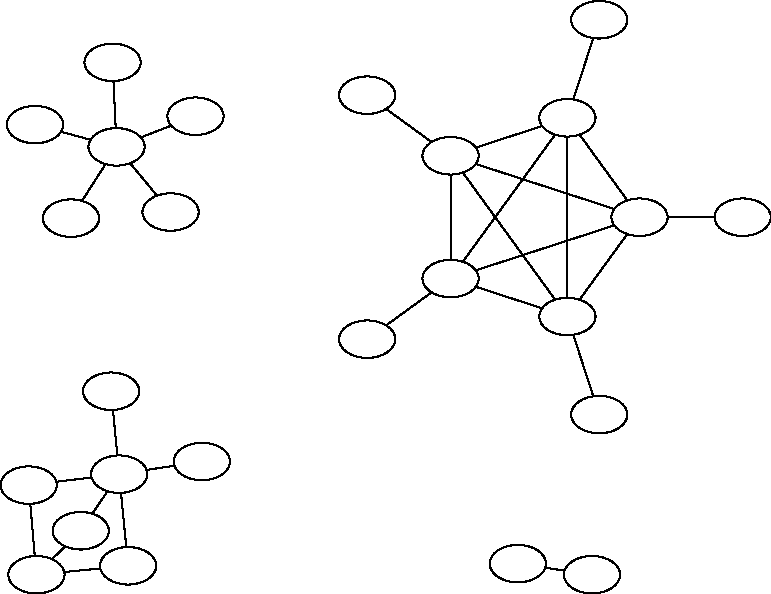
\includegraphics[width=0.9\textwidth]{images/ec2_example.pdf}}

\caption[Chlpaté $2$-hranovo súvislé grafy]{Ukážka štyroch
chlpatých $2$-hranovo súvislých grafov.}

\label{graf:ec2}
\end{figure}

Trieda grafov, ktoré nevieme podľa predošlého dôsledku rozdeliť, obsahuje aj grafy,
v ktorých každý most spája jediný vrchol so zvyškom grafu. Niekoľko takýchto grafov je
znázornených na obrázku \ref{graf:ec2}.

\begin{defn}
    Graf $G$ budeme nazývať \emph{chlpatý $2$-hranovo súvislý graf}, ak je súvislý a pre
    každú mostovú hranu $e \in E(G)$ platí, že jeden z komponentov súvislosti grafu
    $G - \{e\}$ obsahuje jeden vrchol.
\end{defn}

Pripomeňme si, že každý graf, bez ohľadu na jeho štruktúru, má triviálne $L(2,1)$-farbenie
s rozsahom $2n - 2$, kde každému vrcholu priradíme rôzne párne číslo. Pokiaľ pri rozdelení
grafu na dva komponenty ostane jeden z nich dostatočne malý v porovnaní s hodnotou $k$,
pre každé ohodnotenie mostových vrcholov vieme nájsť jeho triviálne $k$-$L(2,1)$-farbenie.
Tento fakt zachytáva nasledujúce tvrdenie.

\begin{lema}
    Nech $e$ je mostová hrana grafu $G$, nech $u_1, u_2$ sú vrcholy incidentné s $e$,
    nech $G_1, G_2$ sú komponenty grafu $G - e$, nech vrchol $u_1$ leží v komponente $G_1$ a vrchol $u_2$
    v komponente $G_2$ a
    nech $n_1$ je počet vrcholov komponentu $G_1$. Ak $2n_1 \leq k$, tak $k$-$L(2,1)$-farbenie
    grafu $G$ existuje práve vtedy, ak existuje $k$-$L(2,1)$-farbenie grafu $G_2 \cup \{e, u_1\}$.
\end{lema}

\begin{proof}
    Implikácia $\boxed{\Rightarrow}$ triviálne platí, dokazovať budeme iba $\boxed{\Leftarrow}$.

    Ukážeme, že ľubovoľné $k$-$L(2,1)$-farbenie $f$ grafu $G_2 \cup \{e, u_1\}$ vieme doplniť na
    $k$-$L(2,1)$-farbenie grafu $G$ s tým, že použijeme iba hodnoty z množiny $\{0, 1, \ldots, 2n_1\}$.
    Presnejšie, dokážeme existenciu množiny farieb $F$ obsahujúcu $f(u_1)$, neobsahujúcu $f(u_2)$,
    v ktorej rozdiel každej dvojice prvkov bude aspoň $2$ a ktorej veľkosť bude aspoň $n_1$.
    
    Graf $G_1$ má $n_1$ vrcholov, vrchol $u_1$ z neho už má priradenú niektorú farbu z $F$. Keď vrcholom
    grafu $G_1 - \{u_1\}$ ľubovoľne priradíme rôzne hodnoty z $F - \{f(u_1)\}$, dostaneme $k$-$L(2,1)$-farbenie
    grafu $G$.

    Rozoberieme niekoľko prípadov:

    \begin{description}
        \item[$\boxed{f(u_1) \not\equiv f(u_2) \pmod{2}}:$] 
            Ak je $f(u_1)$ párne, vezmeme $F = \{0, 2, 4, \ldots, 2n_1\}$.
            Ak je $f(u_1)$ nepárne, vezmeme $F = \{1, 3, 5, \ldots, 2n_1 - 1\}$. V oboch prípadoch majú všetky
            čísla v $F$ inú paritu, ako $f(u_2)$, čiže $f(u_2) \notin F$. Zároveň je veľkosť $F$ aspoň $n_1$.

        \item[$\boxed{f(u_1) \equiv f(u_2) \pmod{2} \wedge f(u_1) < f(u_2)}:$]
            Ak je $f(u_2)$ párne, použijeme množinu
            $F = \{0, 2, \ldots, f(u_1), f(u_1) + 3, f(u_1) + 5, \ldots, 2n_1 - 1\}$. Všetky čísla v $F$, ktoré sú
            väčšie, ako $f(u_2)$, majú inú paritu než $f(u_2)$.

            Podobne pre nepárne $f(u_2)$ použijeme množinu $F = \{1, 3, \ldots, f(u_1), f(u_1) + 3, \\ f(u_1) + 5, \ldots, 2n\}$.

        \item[$\boxed{f(u_1) \equiv f(u_2) \pmod{2} \wedge f(u_1) > f(u_2)}:$]
            Analogicky k predošlému prípadu, pre párne $f(u_2)$ použijeme množinu $F = \{1, 3, \ldots, f(u_1) - 3, f(u_1), f(u_1) + 2, \ldots, 2n_1\}$
            a pre nepárne $f(u_2)$ množinu $\{0, 2, \ldots, f(u_1) - 3, f(u_1), f(u_1) + 2, \ldots, 2n_1 - 1\}$. \qedhere
    \end{description}
\end{proof}

Pokiaľ overujeme existenciu $k$-$L(2,1)$-farbenia pre dostatočne veľkú hodnotu $k$ a v grafe
nájdeme most, ktorého odstránením bude prvý komponent malý a druhý veľký, podľa tejto lemy
môžeme malý komponent odignorovať. Pri takomto prístupe by nám mohli robiť problém malé
hodnoty $k$. Tie môžeme vyriešiť s použitím algoritmu od Haveta a kol., ktorý rieši
problém $k$-$L(2,1)$-farbenia pre $k \leq 5$ v čase $O^*(2.5^n)$ \cite{havet}. Tento
algoritmus principiálne prehľadáva všetky $k$-$L(2,1)$-farbenia grafu, preto sa dá
priamočiaro prerobiť na algoritmus, ktorý rieši problém zoznamového $k$-$L(2,1)$-farbenia.

Teraz máme všetky podklady pre to, aby sme vedeli upraviť algoritmus,
ktorý rieši problém zoznamového $k$-$L(2,1)$-farbenia na chlpatých
$2$-hranovo súvislých grafoch, na algoritmus riešiaci tento problém
na súvislých grafoch.

\begin{veta}
    Ak existuje algoritmus $\mathcal{B}$, ktorý rieši rozhodovací problém zoznamového $k$-$L(2,1)$-farbenia
    na chlpatých $2$-hranovo-súvislých grafoch s časovou zložitosťou $O^*(\alpha^n)$, kde
    $\alpha \ge 2.5$, tak existuje algoritmus $\mathcal{A}$, ktorý rieši problém zoznamového $k$-$L(2,1)$-farbenia
    na súvislých grafoch s časovou zložitosťou $O^*(\alpha^n)$.
\end{veta}

\begin{proof}
    Najprv skonštruujeme algoritmus $\mathcal{A}$, ktorý dostane hodnotu $k$, graf $G$ a zoznam
    povolených hodnôt $c$. Algoritmus bude fungovať nasledovne:

    \begin{enumerate}
        \item Ak $k \leq 5$, spusti algoritmus od Haveta a kol.
        \item Ak $G$ je chlpatý $2$-hranovo-súvislý graf, spusti a vráť výstup algoritmu $\mathcal{B}$.
        \item Inak sa v grafe nachádza netriviálny most. Nájdi most $e$ s koncovými vrcholmi $u, v$.
        Skonštruuj graf $G_1$ ako komponent súvislosti grafu $G - \{e\}$ obsahujúci $u$ a $G_2$ ako
        komponent súvislosti obsahujúci $v$. Bez ujmy na všeobecnosti platí $|V(G_1)| \leq |V(G_2)|$.
        \item Ak $\left |V(G_1) \right| \leq \frac{k}{2}$, rekurzívne spusti a vráť výstup algoritmu
        $\mathcal{A}$ na grafe $G_2 \cup \{e, u\}$ s príslušne zúženým zoznamom hodnôt $c$.
        \item Pre všetky prípustné (podľa $c$) ofarbenia $f$ vrcholov $u, v$ spusti rekurzívne
        algoritmus $\mathcal{A}$ na grafe $G_1 \cup \{e, v\}$. V každom volaní je zoznam $c$ zúžený
        na príslušnú množinu vrcholov a navyše $c(u) = \{f(u)\}$ a $c(v) = \{f(v)\}$. Zoznam dvojíc
        $(f(u), f(v))$, pre ktoré výpočet akceptoval, označíme $Z$.
        \item Pre všetky prípustné (podľa $c$) ofarbenie $f(u)$ vrchola $u$ spusti rekurzívne
        algoritmus $\mathcal{A}$ na grafe $G_2 \cup \{e, u\}$. V každom volaní je zoznam $c$ zúžený
        na príslušnú množinu vrcholov a navyše $c(u) = \{f(u)\}$ a $c(v) = \{x | (f(u), x) \in Z\}$.
        \item Ak aspoň jedno z rekurzívnych volaní v 6. kroku akceptovalo, akceptuj. V opačnom prípade
        zamietni.
    \end{enumerate}

    Overenie, či graf patrí do triedy chlpatých $2$-hranovo-súvislých grafov, vieme realizovať v čase
    $O(|V(G)| + |E(G)|)$ nájdením všetkých mostov pomocou Tarjanovho
    algoritmu \cite{tarjan_bridge}. Prehľadávaním do hĺbky vieme v čase $O(|V(G)| + |E(G)|)$ pre
    každý most a pre každý komponent, ktorý jeho odstránenie indukuje, spočítať, koľko vrcholov obsahuje.

    Pokiaľ platí podmienka v kroku 1, alebo v kroku 2, časová zložitosť algoritmu je nanajvýš
    $T(n) \leq O(|V(G)| + E(G)|) + O^*(\alpha^n)$.

    Pokiaľ sa vykoná krok 4, graf $G_2$ bude obsahovať nanajvýš $n-1$ vrcholov, z čoho dostávame
    rekurentný vzťah pre časovú zložitosť $T(n) \leq O(|V(G)| + |E(G)|) + T(n-1)$.

    Pre každú hodnotu $k \ge 6$ platí, že počet usporiadaných dvojíc farieb, ktorými môžeme
    ofarbiť dva susedné vrcholy, je presne $k(k-1)$. Počet vrcholov grafu $G_1$ označíme $n_1$.

    Krok 5 zahŕňa $k(k-1)$ spustení algoritmu na grafe $G_1 \cup \{e, v\}$, ktorý má $n_1 + 1$
    vrcholov. Krok 6 zahŕňa nanajvýš $k+1$ spustení algoritmu na grafe $G_2 \cup \{e, u\}$, ktorý
    má $n - n_1 + 1$ vrcholov. Časová zložitosť tejto vetvy výpočtu teda spĺňa rekurenciu $T(n) \leq O(|V(G)| + |E(G)|) + k(k-1)T(n_1+1) + (k+1)T(n - n_1 + 1)$.

    Ďalej indukciou dokážeme, že pre vhodne zvolený polynóm $q(n)$ je časová zložitosť
    algoritmu $\mathcal{A}$ nanajvýš $q(n) \alpha^n + O^*(1)$.

    Nech $p$ je polynóm, pre ktorý platí, že časová zložitosť algoritmu $\mathcal{B}$ aj algoritmu
    od Haveta a kol. je zhora ohraničená $p(n)\alpha^n$.

\end{proof}
